\documentclass[unknownkeysallowed]{beamer}

\mode<presentation> {

\usetheme{Madrid}

}

\usepackage{graphicx} % Allows including images
\usepackage{booktabs} % Allows the use of \toprule, \midrule and \bottomrule in tables

\usepackage[slovene]{babel}
\usepackage[utf8]{inputenc}

\usepackage{algorithmicx, algpseudocode}

\usepackage{varwidth}

\algrenewcommand\alglinenumber[1]{\scriptsize #1:}

\renewcommand{\algorithmicrequire}{{\bf Vhod:}}

\def\R{\mathbb R}
\def\N{\mathbb N}

%----------------------------------------------------------------------------------------
%	TITLE PAGE
%----------------------------------------------------------------------------------------

\title[Metoda hibridnih izrezkov]{Računanje presečišč Bezierjevih krivulj z metodo hibridnih izrezkov} % The short title appears at the bottom of every slide, the full title is only on the title page

\author{Domen Keglevič} % Your name
\institute[] % Your institution as it will appear on the bottom of every slide, may be shorthand to save space
{
Fakulteta za matematiko in fiziko \\ % Your institution for the title page
\medskip
%\textit{john@smith.com} % Your email address
}
\date{\today} % Date, can be changed to a custom date


\begin{document}

\begin{frame}
\titlepage % Print the title page as the first slide
\end{frame}

\section{First Section} % Sections can be created in order to organize your presentation into discrete blocks, all sections and subsections are automatically printed in the table of contents as an overview of the talk
%------------------------------------------------

\subsection{Subsection Example} % A subsection can be created just before a set of slides with a common theme to further break down your presentation into chunks

\begin{frame}
\frametitle{Opis problema} 
\begin{block}{Problem}

Dani sta dve ravninski Bezierjevi krivulji ${\bf f}: [\alpha,\beta]\rightarrow \R ^2$ in ${\bf g}:[\xi,\eta]\rightarrow \R^2$. Želimo najti njuna presečišča.

\medskip

Drugače povedano: želimo najti algoritem, ki za poljuben $\epsilon >0$ vrne pare intervalov $[\alpha _i,\beta _i]$ in  $[\xi _i, \eta _i]$, ki vsebujejo presečišča, tako da velja $|\alpha _i - \beta _i| < \epsilon$ in  $|\xi _i - \eta _i| < \epsilon$.
\end{block}
\end{frame}


\begin{frame}
\frametitle{Ideja rešitve}
\begin{columns}[c]
\column{.5\textwidth}
	\begin{itemize}
		\item Krivuljo ${\bf g}$ omejimo z območjem $L$, ki ga omejujejo premice ({\em fat line}).
		\medskip
		\item Krivuljo ${\bf f}$ omejimo z območjem $P$, ki ga dobimo s pomočjo aproksimacije krivulje ${\bf f}$ s krivuljo nižje stopnje ({\em fat curve}).
		\medskip
		\item Omejimo iskanje rešitve na presek območja $P$ in $L$.
		\medskip
		\item Ponavljamo.
	\end{itemize}
\column{.5\textwidth}
	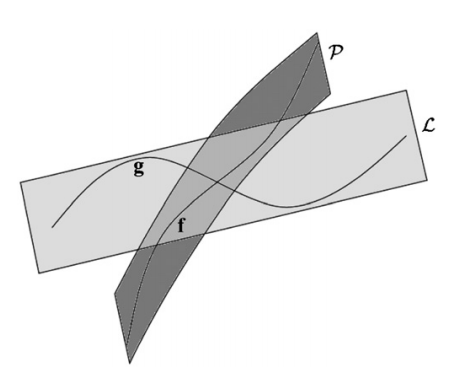
\includegraphics[width=0.9\linewidth,frame]{2}
\end{columns}
\end{frame}

\begin{frame}
\frametitle{Pas okrog $g$ ({\em fat line})}
\begin{columns}[c]
\column{.5\textwidth}
	\begin{itemize}
		\item ${\bf g}(s) = \sum _{i=0}^m{\bf b_i}B_i^m(s)$
		\medskip
		\item Potegnemo vzporednici od premice ${\bf b_0b_m}$ skozi najbolj oddaljeno kontrolno točko na obeh straneh.
		\medskip
		\item Krivulja ${\bf g}$ je vsebovana v pasu med premicama, saj je vsebovana v konveksni ovojnici 
		kontrolnih točk.
	\end{itemize}
\column{.5\textwidth}
	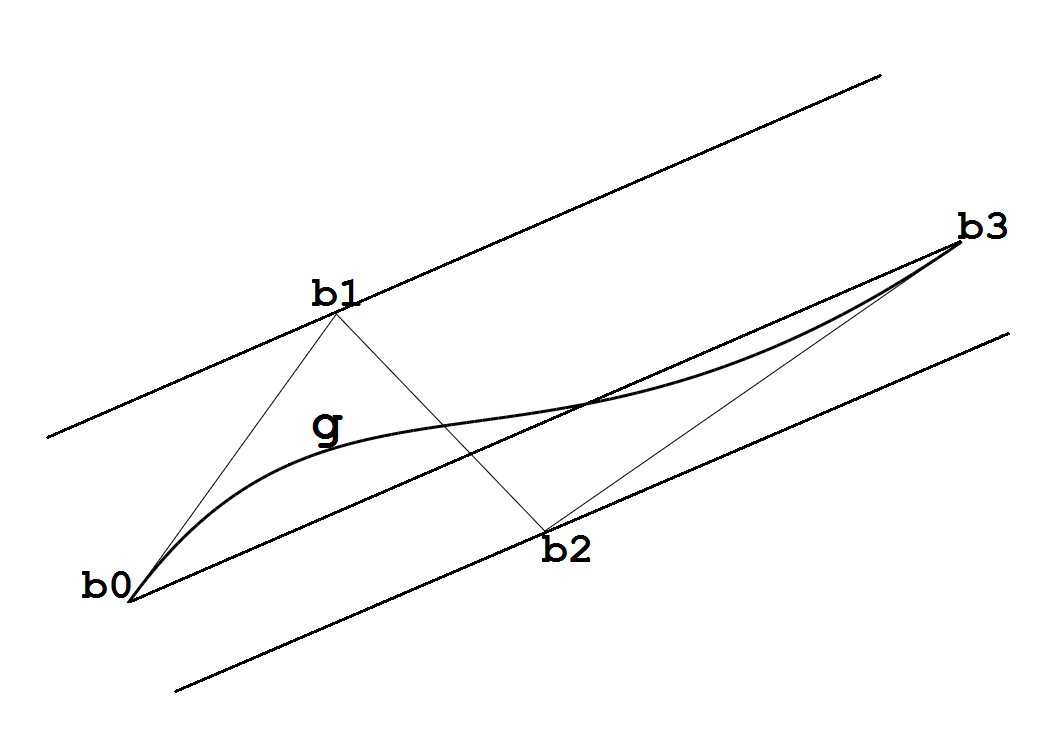
\includegraphics[width=0.9\linewidth,frame]{fat_line}
\end{columns}
\end{frame}

\begin{frame}
\frametitle{Pas okrog $f$ ({\em fat curve})}
\begin{columns}[c]
\column{.5\textwidth}
	\begin{itemize}
		\item ${\bf f}(t) = \sum _{i=0}^n{\bf a_i}B_i^n(t)$
		\medskip
		\item Z nižanjem stopnje aproksimiramo ${\bf f}$ s krivuljo ${\bf p}$ stopnje $k$.
		\medskip
		\item $\lVert {\bf f} \rVert _{BB} = \max _{i = 0,\ldots,n} \lVert {\bf a_i} \rVert $ je norma.
		\medskip
		\item Za $\delta = \lVert {\bf f}(t) - {\bf \tilde{p}}(t) \rVert _{BB}$ je $\lVert {\bf f}(t) - {\bf p}(t) \rVert \leq \delta$.
	\end{itemize}
\column{.5\textwidth}
	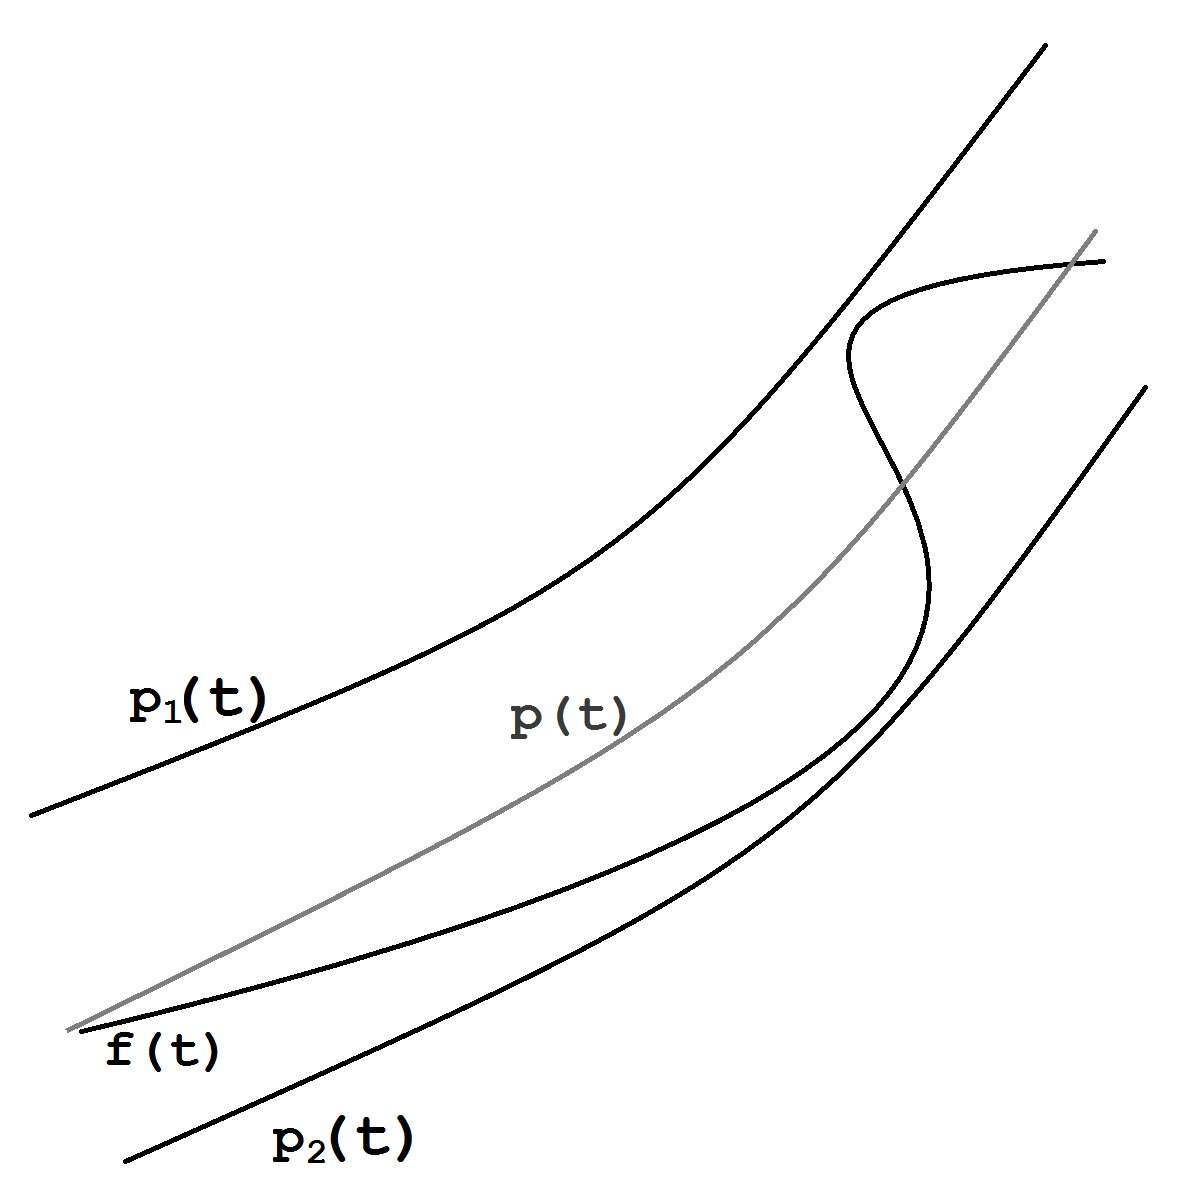
\includegraphics[width=0.9\linewidth,frame]{fat_curve}
\end{columns}
\end{frame}

\begin{frame}
\frametitle{Iskanje intervalov}
\begin{small}
Naj bodo ${\bf b_i}$ kontrolne točke Bezierjeve krivulje ${\bf g}$ in ${\bf n}$ normala na ${\bf b_0b_m}$. Definiramo
\medskip
$$
{\bf p_1}(t) = {\bf p}(t) + \delta {\bf n} 
$$
$$
{\bf p_2}(t) = {\bf p}(t) - \delta {\bf n}
$$
$$
d_{max} = \max _{i=0,1,\ldots,m}\{ {\bf n}\cdot({\bf b_i}-{\bf b_0})\},
$$
$$
d_{min} = \min _{i=0,1,\ldots,m} \{ {\bf n}\cdot({\bf b_i}-{\bf b_0})\} ,
$$
$$
d_1(t) = {\bf n}\cdot ({\bf p_1}(t) - {\bf b_0}),
$$
$$
d_2(t) = {\bf n}\cdot ({\bf p_2}(t) - {\bf b_0}).
$$
Iskana presečišča so rešitve enačb $d_1(t) = d_{min}$ in $d_2(t) = d_{max}$.
\end{small}
\end{frame}

%------------------------------------------------


\begin{frame}
\frametitle{Psevdo koda}

\begin{scriptsize}
   \begin{algorithmic}[1]
	\Require $({\bf f},{\bf g}, [\alpha,\beta], [\xi,\eta], k)$ : ravninski Bezierjevi krivulji, njuni domeni in stopnja apr. krivulje

	\If{$|\alpha - \beta | < \epsilon$ in  $|\xi - \eta| < \epsilon$}
		\State \Return $([\alpha,\beta],[\xi,\eta])$
	\Else
		
		\If{$|\alpha - \beta | \geq |\xi - \eta|$}
			\State $L, P \gets $ raven pas okrog ${\bf g}$ ({\em fat line}), ukrivljen pas okrog ${\bf f}$ ({\em fat curve})
			\State Najdi intervale $[\alpha _i,\beta _i]$, kjer je $L\cap P\neq \emptyset$
			\If{$l > 0$ in $\max _{i=1,\ldots ,l}\, \{ |\alpha _i - \beta _i|\} \geq 
				\frac{1}{2}|\alpha -\beta |$}
				\State \Return \begin{varwidth}[t]{\linewidth} 
					$HybridClip({\bf f},{\bf g},[\alpha,\frac{1}{2}(\alpha+\beta)],[\xi,\frac{1}{2}(\xi+\eta)],k)$\par$
        \hskip\algorithmicindent
					\cup \, HybridClip({\bf f},{\bf g},[\alpha,\frac{1}{2}(\alpha+\beta)],[\frac{1}{2}(\xi+\eta), \eta],k)$\par$
        \hskip\algorithmicindent
					\cup \, HybridClip({\bf f},{\bf g},[\frac{1}{2}(\alpha+\beta), \beta],[\frac{1}{2}(\xi+\eta), \eta],k)$\par$
        \hskip\algorithmicindent
					\cup \, HybridClip({\bf f},{\bf g},[\frac{1}{2}(\alpha+\beta), \beta],[\xi, \frac{1}{2}(\xi+\eta)],k)$
					\end{varwidth}
			\Else
				\State $S\gets \emptyset$

				\For{$i=1,\ldots,l$}
					\State $S\gets S\cup HybridClip({\bf f},{\bf g},[\alpha _i,\beta _i], [\xi,\eta],k)$
				\EndFor
				\State \Return $S$
			\EndIf
		\Else
			\State $HybridClip( {\bf g}, {\bf f}, [\xi,\eta],[\alpha,\beta],k)$
		\EndIf
	\EndIf

   \end{algorithmic}
\end{scriptsize}

\end{frame}


\begin{frame}
\frametitle{Opombe}
\begin{itemize}
\item Krivuljo ${\bf f}$ aproksimiramo s krivuljo stopnje $2$ ali $3$, saj v tem primeru ničle lahko najdemo analitično.
\medskip
\item Algoritem nima začetnih pogojev od katerih bi bil odvisen (npr. izbire začetne točke).
\medskip
\item Če sta krivulji zelo blizu, potem lahko vrne napačen rezultat (najde presečišče, ki ga ni).
\medskip
\item V primeru tangentnih presečišč se obnaša kot {\em divide and conquer}.
\medskip
\item Konvergenca za transverzalna presečišča je vsaj kvadratična.
\end{itemize}
\end{frame}

%------------------------------------------------

\begin{frame}
\frametitle{Red konvergence}
\begin{small}
\begin{block}{Lema 1}
Naj bo ${\bf f}$ Bezierjeva krivulja stopnje $n$. Potem obstaja konstanta $C$, da za poljuben interval $[\alpha,\beta]\subset[0,1]$ velja $\delta \leq C |\alpha - \beta|^{k+1}$.
\end{block}

\begin{block}{Lema 2}
Naj bo ${\bf f}$ Bezierjeva krivulja stopnje $n$. Potem obstajajo konstante $C_{j}$, da za poljuben interval $[\alpha,\beta]\subset[0,1]$ in optimalno aproksimacijo ${\bf p}$ stopnje $k$ od ${\bf f}$ velja
$\lVert {\bf f}^{(j)} - {\bf p}^{(j)} \rVert _{\infty} \leq C_{j}|\alpha - \beta|^{k+1-j}$, za $j=0,1,\ldots,k$. 
\end{block}

\begin{block}{Trditev}
Naj imata Bezierjevi krivulji ${\bf f}$ in ${\bf g}$ transverzalno presečišče v ${\bf f}(t_0)={\bf g}(s_0)$. Potem obstajajo konstante $C_f, C_f', C_g$ in $C_g'$, da za dovolj velike $i\in \N$ velja
$$
|\alpha _{i+1} - \beta _{i+1}| \leq C_f |\alpha _{i} - \beta _{i}|^{k+1} + C_g|\xi _{i} - \eta _{i}|^2
$$
oz.
$$
|\xi _{i+1} - \eta _{i+1}| \leq C_f' |\alpha _{i} - \beta _{i}|^{2} + C_g'|\xi _{i} - \eta _{i}|^{k+1}.
$$

\end{block}
\end{small}
\end{frame}

\begin{frame}
\frametitle{Primeri}
\center
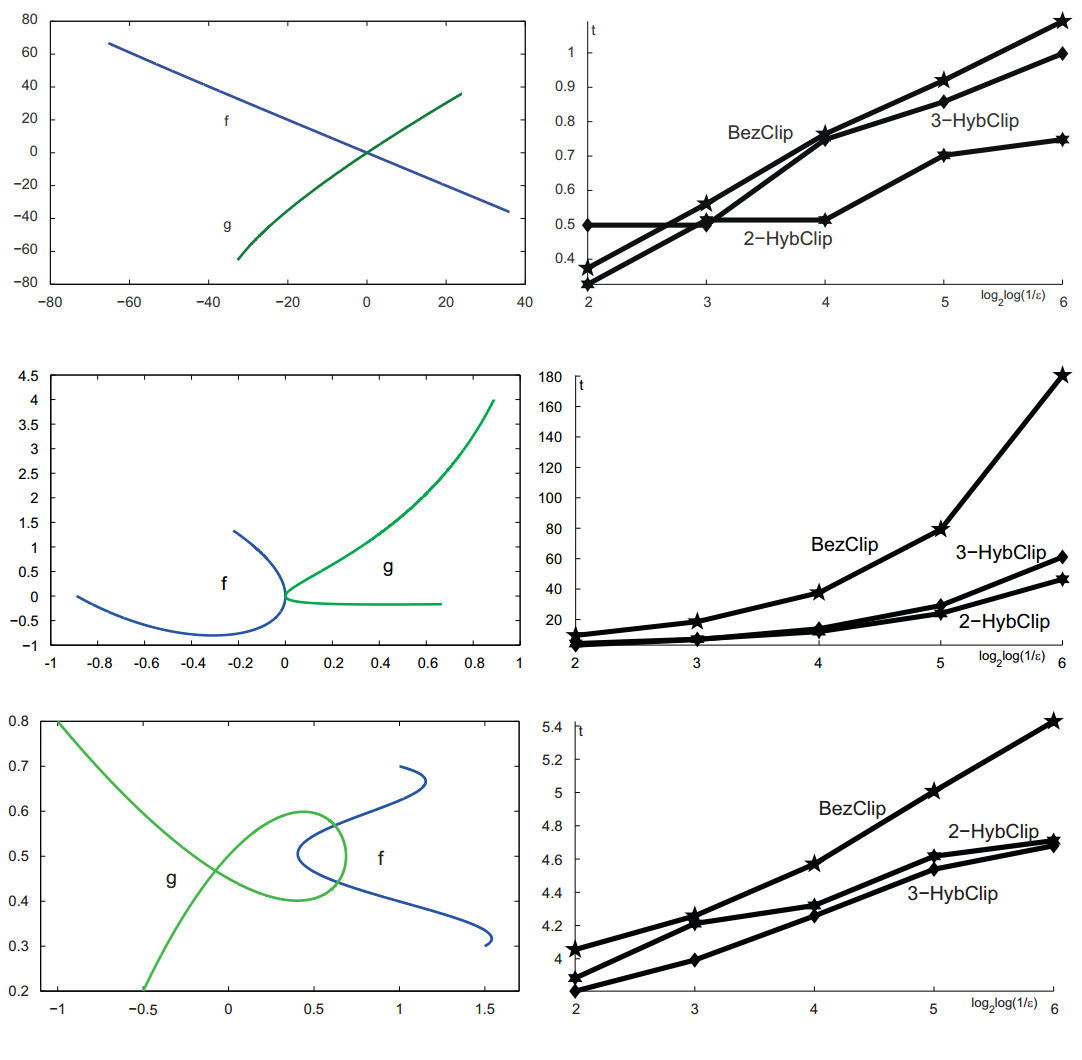
\includegraphics[width=0.6\linewidth,frame]{primeri}
\end{frame}

%------------------------------------------------

\begin{frame}{Konec}
\Huge{\centerline{Konec}}
\end{frame}

%----------------------------------------------------------------------------------------

\end{document}